\documentclass[table,a4paper,oneside]{book}

\usepackage{graphicx} % Allows insert of graphics
\usepackage{longtable} % Allows for multipage spanning tables
\usepackage{pdfpages} % Simplifies insertion of multipage PDF’s
\usepackage{natbib} % Puts in bibliography style
\usepackage[pdfborder=0 0 0]{hyperref} % Adds PDF links
\usepackage{mathptm} % Changes font
\usepackage{fancyhdr} % Allows the use of the fancy Header package
\usepackage{url} % Makes URL’s appear nicer and follow formatting rules
\usepackage{algorithm} % Allows Algorithmic insertions to be floated
\usepackage{algorithmic} % Allows Algorithms and Pseudocode
\usepackage{textcomp} % LaTeX support for the Text Companion fonts.
\usepackage{setspace} % Allows the use of the set space command
\usepackage{listings} % Allows the use of source code
\usepackage{colortbl} % Adds colour to rows etc
\usepackage{acronym} % Allows the use of acronyms in code - deals with printing acronyms out nicely
\usepackage[a4paper,vmargin={25.4mm,25.4mm},hmargin={25.4mm,25.4mm}]{geometry} % Allows the changing of page borders

\setlength{\parindent}{0.0in} % Sets paragraph indentation to 0
\pagestyle{fancy}
\bibpunct{(}{)}{,}{a}{,}{,} % Defining the citation style
\newcommand{\degree}{\ensuremath{^\circ}} % Sets new command - Inserts degree symbol
\newcommand{\HRule}{\rule{\linewidth}{0.5mm}} % Set new command - Add blank line
\newcommand{\mtwo}{m\textsuperscript{2} } % Sets the command - Adds m^2.

% Acronym Definition
% \acrodef{label}[acronym]{written out form}
% \acrodef{acronym}{written our form}
\acrodef{ADB}{Approved Document B}
\acrodef{BCIS}{Building Cost Information Service}
\acrodef{CLG}{Department of Communities and Local Government}
\acrodef{CSV}{Comma Seperated Value}
\acrodef{FPA}{Fire Protection Association}
\acrodef{FRS}{Fire and Rescue Service}
\acrodef{IRS}{Incident Reporting System}
\acrodef{IRMP}{Integrated Risk Mangement Plan}

\begin{document}
\chapter{Literature Review}

\section{Introduction}
\subsection{Background}
Fire has posed a risk to life and property ever since it was discovered.  Throughout history, fire has been the cause of many injuries, deaths and property loss.  Large fires, such as the Great Fire of London, caused massive widespread damage to entire cities and fires such as these led to the initial development of fire codes and regulations \citep{Stollard1994}.
\\
\\
Over the years, these rules and regulations have changed and evolved, especially after major fires have occurred. These changing rules and regulations have led to the development of the current building codes that are in place today.
\subsection{Aims and Objectives}
The aim of the following research is to investigate and make recommendations on the passive fire protection in commercial, public and heritage buildings.
\\
\\
This will be achieved by meeting various objectives. These objectives are detailed below.
\begin{itemize}
\item Conduct a literature review of previous and current research
\item Conduct a review of current design practices
\item Recommend changes in the fire engineering design process to decrease reliance on active systems
\end{itemize}
\section{Methodology}
\subsubsection{Literature Review}
The literature review is designed to discover the current state of research in the fire design area and the uses of fire protection in the industry. Undertaking the literature review will allow areas of further research to be identified. This will be achieved by reading building codes and regulations, research papers in journals and recent books in the fire engineering area.
\subsubsection{Current Practice}
\textbf{Investigate the Fire Engineering Design Process}
\\
The fire engineering design process will be investigated in detail so that an understanding of how a fire engineered solution is designed, proposed and accepted by building control. This will give me an idea of how the fire engineered design solution is accepted and what compromises may have to be taken on board by both building control and the fire engineers in charge of the design. This will be achieved by interviews and questionnaires with both fire engineers and building control.
\\
\\
\textbf{Identify Passive Fire Protection in Use}
\\
In this section, the current state and use of passive fire protection in the construction industry will be investigated. It will tell me what passive fire protection measures are used and where within the trade. This will be done partly in the literature review and also with questionnaires and interviews with fire engineers and architects.
\\
\\
\textbf{Identify Where Protection Is Required}
\\
This section will look at where passive fire protection is used in buildings and if this is the right place for use.  This will show where the protection is currently used and for what purpose. This will be achieved in the literature review and with questionnaires and interviews with fire engineering professionals.
\\
\\
\textbf{Understand How Passive Fire Protection is Chosen}
\\
Once the passive fire protection is identified, what affects the choice of different passive measures in different locations needs to be investigated. This will give an indication of what designers, architects and clients want and where and if there are any other viable alternatives. This will be achieved with interviews and questionnaires and looking at rules and regulations.
\\
\\
\textbf{Costs of Passive Fire Protection}
\\
Once the passive fire protection measures, locations and how they are chosen have been identified, then the costs of the fire protection measures that are installed can be identified. This will comparison of the costs of each individual protection measure. This can be achieved by contacting the manufacturers and suppliers of the fire protection measures.
\\
\\
\textbf{Effectiveness of Passive Fire Protection Measures}
\\
Once the passive fire protection measures have been identified, the effectiveness of passive fire protection, once installed within buildings, can be investigated. This will allow comparison between different passive fire protection methods and active measures. This will be achieved by looking at data from fires, results from previous research, fires tests and questionnaires to fire the service and fire engineers.
\\
\\
\textbf{Cost Effectiveness of Fire Protection Measures}
\\
With the effectiveness and cost gathered from previous steps, the cost effectiveness of each protection measure can be studied and looked at. This will be calculated from the costs of fitting and the effectiveness of passive fire protection.

\subsection{Current Legalisation}
Even with fire engineering approaches, the majority of building designs will take various aspects from the rules and regulations. However, ``cherry picking'' (choosing bits that suit the project from different fire codes and using that) is generally considered bad engineering and under newer standards (BS 9999), discouraged.
Knowing the basics of the rules, regulations and standards is needed to look at fire engineering principles and fire protection methods as a knowledge of what is required is needed. Therefore the differences between regulations, standards and codes are addressed below.
\\
\\
In the UK, there are various codes and management regulations that need to be followed to prove that a premises is deemed fire safe. Some of this legalisation is put into effect when the building is constructed; others are only taken into account once the premises have been occupied and being used.
\subsubsection{Regulations}
In the UK, buildings have to be built to achieve the requirements laid down in the building regulations but as long as the building can achieve these requirements, they can be met in any way.
\\
The regulations are split into many different areas, concerning various aspects, such as fire safety and toxic products. As the building regulations are large and complex, the Communities and Local Government have published a series of approved documents, each split down into topic areas that need to be covered and the easiest way for a building in the UK to achieve a building regulation compliant design is to follow the guidelines laid down in these documents. The one relating to fire safety is Approved Document B: Fire Safety (ADB) and this details basic layouts and basic guidelines for the application of fire safety in buildings. It is realised that the guidelines in this document are firstly very prescriptive and secondly, they result in simple, basic buildings and that if an architect wishes to build a more innovative building, then ADB will restrict this.
\subsubsection{Standards}
Standards describe the British Standards, set by the BSI (British Standards Institution), which specifies the performance and safety requirements of a product or system. Two British standards also provide an alternative method of meeting the building regulations with regards to fire,  `BS 9999: Code of Practice for Fire Safety in the Design Management and Use of Buildings' and `BS 7974: Application of fire safety engineering principles to the design of buildings: Code of practice'. These two standards lay down the requirements for meeting the building regulations without using ADB whilst other British standards relate to equipment and construction within the building - ADB, BS 9999 and BS 7974 require equipment within a building to have achieved a level of performance described within the relevant British standard.
\\
BS 7974 is a complete fire engineering based solution from first principles and it is used on the most innovative buildings, where they are unable to follow the guidelines in ADB to achieve the level of design the building architect wants. In this case, the rules within BS 7974 are followed to achieve a design that is based on performance design. Fire is studied from it's beginning and the whole building is designed around this, to satisfy the building regulations.
BS 9999 is a mid point between ADB and BS 7974. When a designer wishes to make his design more complicated than ADB but the design is not sufficiently complex to use BS 7974 then BS 9999 can be used as a compromise between the two. BS 9999 is almost, but not quite, a performance based code as it takes into account the occupancy of the building it is being installed in and specifies various solutions based on the risk profile of a building. This allows different designs to accommodate for differing levels of risk within the property, something that ADB does not differentiate between - in ADB, for example, all industry buildings are deemed to be the same fire risk, regardless of what industrial activity takes place within the buildings.  For instance, the fire risks within a polystyrene factory and a furniture factory aren't the same - a fire in the polystyrene factory will ignite and spread more easily than in a furniture factory and as BS 9999 takes this into account, the design for the furniture factory will be able to have extra benefits over the polystyrene factory such as larger compartment sizes due to the lower fire risk.
\subsubsection{Codes}
Codes are the American version of the building regulations however the term is often used to describe the British building regulations as well. In America, the rules and regulations differ. In each state (and sometimes cities,  New York City for example), there is an individual building code. This code is generally based off the International Building Code (IBC) with the state adding its own requirements and clauses. However the state code may not be updated as often as the IBC. Therefore in each state you must comply with the state building code, which will typically reference other codes such as NFPA 101 `Life Safety Code'.
\subsubsection{Regulatory Reform (Fire Safety) Order}
Once a building is built and is occupied, it has to regularly be checked to make sure that the building remains fire safe.  Hazards, such as occupants blocking escape routes, need to be found and corrected. This used to be undertaken by the fire service until the introduction of the Regulatory Reform (Fire Safety) Order, (known from here on as the RRO) in 2005.
Under the RRO, non domestic properties have to nominate a person as the ``responsible person'' and it is the responsible persons duty to ensure that a risk assessment is carried out for the premises that they are responsible for and steps are taken to reduce any fire risk highlighted by the risk assessment.
\\
\\
The RRO took many previous but different legalisation and regulations and combined them together to make it easier for businesses and enforcing authorities to follow and comply. It focuses on performance based criteria rather than the previously prescriptive based legalisation that was used and this places a greater onus on the business to comply with the legislation than before, due to the risk assessments needed for the property.
Prevention as they say, is better than cure, and the RRO is seen as a step towards preventing fires occurring, thus allowing savings on fire fighter call outs and associated costs.
\\
\\
The Government produce a range of guidelines and help documents on the risk assessment methods which are freely available for download on the Communities and Local Government website and these guides detail the outline of the risk assessment process for each different property type that needs to be risk assessed.
\\
\\
It should be noted however that even 3 years after the RRO became law in 2006, that the Fire and Rescue service are finding some premises and buildings are not complying with the RRO or are even unaware of its existence \citep{Communities2009}. This research found that the Fire and Rescue service were reluctant to give help when requested, partly due to their nature of the enforcers of the RRO and it also found that many businesses, especially the smaller businesses did not have any awareness of the Government produced documentation on risk assessments. These results were also confirmed in a survey of the Fire Protection Association members \citep{Wilkinson2008}.
\subsection{Fire Protection Methods and Systems}
Buildings that have fire protection installed are generally not protected by just one fire protection system. Often the fire safety strategy for a property can be made up of 3 or more fire safety systems that form the core fire safety strategy. 
\\
\\
Some fire safety systems are required in the property through either the national building regulations or insurance company requirements. For example, Approved Document B states that all buildings over 30m should be equipped with a sprinkler system \citep{Communities2006}, yet a smaller building may want to install sprinklers to provide additional property protection/insurance premium reduction or as an insurance requirement.
\\
Fire safety measures differ in how they act within the fire safety system. For example, alarms and detectors do not fight the fire themselves but warn occupants of a fire and allow them to escape, where as sprinklers, unless connected to a flow valve, do not automatically alert all occupants within a building that a fire has broken out.
\subsubsection{Smoke Detection and Alarms}
Most buildings except the smallest require a form of alarm system, this is to alert occupants that a fire is occurring within the premises, even if the occupants are not in the room of fire origin. Bigger buildings will have more complex alarm and detection systems that are able to pinpoint exactly where in the building the fire has started by having an addressable alarm system and a display panel which states what detector has detected the fire. This allows the fire service to very quickly locate the area of fire origin and start fire fighting operation as soon as they arrive on scene.
\subsubsection{Sprinklers}
Sprinklers are a means of controlling fires and preventing them from spreading, yet sometimes sprinklers will extinguish the fire before the fire service arrive. However they are primarily designed to keep the fire spread under control, which means the fire service will have a smaller fire to extinguish upon arrival. There are various types of sprinklers systems which differ in operation methods - wet pipe sprinklers are sprinklers where the pipe work contains water at all times and dry pipe sprinklers are sprinklers where the pipe work does not contain water until a sprinkler is activated and then water enters the system. The wet pipe sprinklers are quicker at delivering suppression to the fire; however they are not suitable in cold climates where the water is likely to freeze and cause ruptures in the pipes.
\subsubsection{Compartmentation and Passive Fire Protection}
Compartmentation aims to prevent an entire building conflagration by preventing internal fire spread. This also allows other building occupants to escape (flats for example) and make the fire more manageable for firefighters to extinguish. Compartmentation is achieved by using passive fire protection measures to separate the building into compartments of various size. These compartmentation sizes are specified in ADB for different building uses and a building cannot exceed these compartment dimensions unless the fire engineer can prove to the building control authority that doing so does not compromise the safety of the building.
\\
\\
Passive fire protection are methods of protecting a building that don't require any kind of activation. Examples include fire resistant cladding or intumescent paints, amongst other measures. These passive protection measures are the main material used in compartmentaion and as they degrade under fire conditions, they will prevent the fire from spreading. Passive fire protection measures are rated according to the time they will prevent fire spread through the material and they must be insulating, to prevent heat passing through them and igniting material on the other side of the material and must have structural integrity so that fire products such as smoke and embers cannot penetrate through the protection. Loadbearing walls must also have a loadbearing capacity where it is needed. These three factors form the basis of the rating and the codes will specify where each timing is required.
\subsubsection{Smoke Control and Pressurisation}
Smoke control and pressurisation systems are not generally required in buildings except in certain circumstances, however if they are installed, extra benefits can be given to buildings, such as smaller corridor widths and longer travel distances \citep{BSI2008}. Due to the benefits gained in the building design process due to extra fire systems being installed, part of the cost of installation maybe made up for in increased usable area inside the building.
\\
\\
Smoke from a fire does not remain in the same location as the seat of the fire and smoke will spread throughout the fire compartment and if the compartment is not sealed against smoke flow, it will eventually spread into other compartments. Drysdale covers the factors affecting smoke movement in his book, An Introduction to Fire Dynamics \citep{Drysdale1998}. Smoke moves around the compartment and thus out into the rest of the building via smoke buoyancy, expansion of combustion gases, the stack effect, via wind, the elevator piston effect and finally by heating, ventilation and air conditioning (HVAC) systems. Klote briefly mentions HVAC systems in his chapter in the SFPE Handbook For Fire Protection Engineering \citep{Klote2002}. In fires, HVAC systems are shut off to avoid getting air to the fire and allowing smoke and combustion products to be spread by the air systems. However, smoke will still be able to spread throughout the ducting naturally using the other effects mentioned above. Research has proven that HVAC systems will spread smoke and combustion products round a building faster and in greater concentrations than if the HVAC system was shut off and smoke spread via the other movement methods \citep{Mowrer2004}.
\\
\\
Smoke control systems, known as SHEVS (Smoke and Heat Exhaust Ventilation Systems), can be installed within a building and most buildings over a certain size or height will include some degree of smoke control within them, if only in fire fighting shafts. In ADB, the guidance is that all buildings over 18m require fire fighting shafts and in BS 9999, it is required that all fire fighting shafts over 30m to have a pressure differential system \citep{BSI2008}.
\\
SHEVS can be installed for a variety of reasons. BRE 368 gives a list of design philosophies behind installing a SHEV system \citep{HPMorgan1999}. It suggests:- 
\begin{itemize}
\item Protection of Means of Escape
\item Temperature Control
\item Assisting Fire Fighter Operations
\item Property Protection
\end{itemize}
Protection of means escape is critical and thus the pressurisation systems usually seen, are those within staircases or the smoke reservoirs used in shopping centres to prevent smoke flow along the length of a mall area. Smoke has to be prevented from entering the means of escape from a building where ever possible or if it does enter, it must be kept above head height and ideally, much higher than head height, to prevent escaping occupants being subjected to thermal radiation from the smoke and also from inhaling the toxic products of combustion.
\\
\\
Smoke from the fire is hot and rises. In the open, the smoke is free to be carried away under the fires thermal currents. However in a compartment, the smoke will build up, unless there is a means for it to escape. As it builds up, the area under the smoke is subject to radiative heat flux as the heat from the smoke is radiated downwards and this radiative heat flux will increase as the smoke temperature increases. This is part of the process that leads to flashover in a compartment \citep{Drysdale1998} and therefore if the smoke can be removed from the compartment, the radiative heat flux from the smoke layer will decrease and flashover can be delayed or prevented. This can be used to help protect property - flashover is less likely to occur within the fire compartment with the extraction of the hot combustion gases and thus less structural damage will occur, as the structural integrity of a compartment is impacted in the high intensity fire after flashover \citep{Ramachandran1990}.
\subsubsection{Modelling}
Most large engineering companies will use modelling to help them in the design and engineering of a building during planning and construction. Computer modelling of fire hasn't been used until recent advances in computer technology and computer models have made this possible. Even now, considerable time and effort is needed to design and run the computer model and to interpret the results.
\\
\\
There are various types of fire models available that offer different benefits and drawbacks to the end user. These are split into two types of models, zone models and field models.
\\
Zone models are relatively simple models that can output answers quickly and with relatively little running costs.  However because they are simple models, the results they give are not very accurate and cannot be used to show how smoke and fire is likely to progress throughout a building. Field models on the other hand take much longer to run and thus have a larger running cost but they do provide better estimates of fire growth and smoke movement, due to the many calculations they perform for each field within the model. These computational fluid dynamic models are the models most often used in the application of fire design, thanks to the more accurate results they are able to give. They require more training to use and require that the user knows the essentials of the program and of fire engineering to get and interpret the results from the program \citep{Cox1994123}.
\section{Previous Research}
\subsection{Effectiveness}
All systems within fire safety can be analysed to determine their effectiveness in regards to their role within the system. It should be noted that the effectiveness of an entire system depends upon the effectiveness of the individual components. If an alarm system is classed as very effective but the detection system installed alongside it is not and fails to detect the fire, the effective alarm system has been nullified by ineffective detection system.
\subsubsection{Smoke Detection and Alarms}
One of the most useful detection methods is smoke detection. Simple and easy to install, especially in the home environment. However smoke detection can be prone to false alarms when used in the wrong areas, as depending on the type of smoke detector, it can be activated easily by water vapour, other particles in the air (such as dust) and cooking fumes \citep{XieQiyuan07012004}. False alarms are an annoyance, cause disruption, increase the cost of fire fighting and cost the UK economy �m in 2004 \citep{TheDeputyPrimeMinister2006}.
\\
\\
Smoke alarms have a different effectiveness on different age groups and in a study by Bruck, it was found that children are less likely to wake up for a fire alarm than the parents. \citep{Bruck1999369}. This means that adults will then have to wake the child/children before escaping from the property, wasting time that could be used to escape.
\\
\\
The effectiveness of smoke detectors in Australia has been investigated by He and Nelson in 2008. They investigated the effectiveness of smoke detectors in both commercial properties and in residential dwellings. They found that smoke alarms were more effective in dwellings for adults but if the building occupant interactions are taken into account (such as trained staff working to help evacuate people as well as the alarms) then the commercial alarms were more effective than the dwelling alarms, especially at night, where the dwellings occupants would be asleep \citep{He2008}.
\subsubsection{Sprinklers}
The effectiveness of sprinklers is a crucial element within larger buildings and high rise structures. With a sprinkler system installed, these buildings are allowed additional design space beyond what would normally be allowed if they were not fitted with sprinklers. Therefore if the buildings sprinklers fail to operate or fail to contain the fire, then the building is liable to suffer larger amounts of damage, due to the large floor area or cause risk to occupants within the building that might be relying on the sprinklers to contain the fire and allow them time to escape before conditions within the building become untenable.
\\
Sprinkler systems therefore need to be reliable (operate in a fire) and effective (contain the fire to the designed level). Previous research by Melinek shows that sprinklers are effective in reducing the probability of fires reaching an area greater than 100m\textsuperscript{2}. However they have little effect on the probability of fire spread until the fire has reached 3m\textsuperscript{2}. This suggests that a fire has to reach 3m\textsuperscript{2} before it will be hot enough to activate the sprinkler heads \citep{Melinek1993299}.
\subsubsection{Compartmentation and Passive Fire Protection}
Passive fire protection is one of the easiest methods of protecting against fire spread of fire damage. Passive fire protection is defined by the Factory Mutual Research Corporation \citep{Corporation1991} as the protection through:-
\begin{itemize}
\item High resistance to ignition
\item Slow and/or decelerating fire growth
\item Low heat release rate and generation rates of fire products
\item Short fire duration
\end{itemize}
Examples of passive fire protection are given in ``Ensuring Best Practice for Passive Fire Protection in Buildings'' published by the ASFP (Association for Specialist Fire Protection)  \citep{ASFP2004}. They describe passive fire protection as: -
\begin{enumerate}
\item The basic elements of the structure without any further treatment; eg steelwork, concrete, brickwork
\item The same elements of structure with specialist additional treatment to enhance the fire performance, when the additional treatment has been tested and classified to standardised methods; eg steelwork treated with intumescent paint or boxed/profiled specialist board materials
\item Non-structural systems or materials added between/into elements of structure to ensure that the spread of fire cannot pass around/through the  elements of structure described in 1 and 2; eg insulated fire-resisting partitions, cavity barriers, specialist fire-stopping of gaps in structure or those gaps or holes created when installing building services
\item Materials of construction where the spread of fire over their surfaces is minimal and which exhibit little heat release in fire. These materials do  not exhibit sustained burning from direct ignition or from exposure to radiation from adjacent fires; eg the use of wall lining materials which will not  add fuel to the fire, and which will therefore limit the fire growth
\item Doors
\item Purpose-designed ancillary systems, for example to ensure that fire doors or dampers in ductwork close effectively to prevent the passage of fire
\end{enumerate}
Passive fire protection covers a variety of various applications. Building compartments, built with fire resisting materials, are passive fire protection measures, as is the intumescent paint and other materials used to protect steel beams within buildings. These passive fire protection measures are designed to contain the fire, prevent its spread and prevent damage where possible from fire.
\\
\\
Recently, passive fire protection has been applied to concrete even though concrete is deemed as fire proof. It is a Class 0 material, which means it is non combustible or of limited combustion, and is thus commonly used in escape routes to prevent fire spread \citep{Communities2006}. Due to its wide use throughout the building industry, it has been subjected to fire on many different occasions and has been noted to undergo explosive spalling. This phenomena is seen when concrete is exposed to high temperatures which causes the water within the concrete to vaporise and move to the surface, destroying the concrete. In the Channel Tunnel fire in 1996, various sections of the tunnel suffered severe spalling and in places the concrete was almost reduced to the bedrock \citep{Comeau1997}. Due to spalling like this, passive fire protection has been applied to concrete to prevent the fire causing such damage. Various methods exist to protect concrete, the most effective of which is a thermal barrier \citep{Khoury2008}. The thermal barrier prevents heat reaching the concrete and thus prevents spalling, similair to that of intumescent paint on steel. Another method in Khourys article is the addition of polypropylene fibres to concrete. These do not prevent the temperature of the concrete increasing but can minimise or even prevent explosive spalling from occurring.
\\
\\
Sustainability of buildings is a big design focus at the current time. With good building design, there is less emphasis on using secondary systems in the building such as HVAC systems that use energy and reduce the sustainability of buildings and the use of sustainable construction materials. Fire engineering, even in these sustainable buildings, is still essential if the design does not follow ADB. However research has been done on whether fire protection can be made more sustainable with the use of different and new fire protection materials.  Fly ash from biomass burnt to provide power has some good properties that can be used for fire protection and a methodology has been developed by Vilches et al \citep{Vilches2005776} to test the new and different fly ash pastes that can be made with differing ashes from different biomass fuels. The pastes that perform well can then be further refined to create a panel, similar to plasterboard. Leiva et al have studied the use of internal partition panels made with ash from biomass power stations \citep{Leiva2009622}. They found that the panels had similar performance to that of gypsum plasterboard panels, in both fire conditions and in material properties. This could, in the future, be an alternative material for fire protection within buildings that is sustainable  using waste materials from sustainable power development. 
\\
\\
In the research conducted by Remesh and Tan \citep{K.Remesh09012006}, they found that smoke spread in a non partitioned flat unit was quicker than the smoke spread within a partitioned unit, meaning that the layout of a flat and building can affect the smoke spread and thus affect how quickly tenability limits are reached within a building. The basis of compartmentation is to prevent smoke spread around a building and this research gives a good indication of why compartmentation should be installed within buildings.
\\
\\
Steel beams are a common building material, especially with high rise buildings. However, after the 9\slash11 attacks on the World Trade Centre, a lot of focus has been on protecting steel columns in fires, especially as NIST states that WTC building 7 ``underwent progressive fire induced collapse due to structural failings due to fire'' \citep{NIST2008}. Other fires have caused weakening of steel structural supports and deformed buildings, most notably the Broadgate Phase 8 fire in London, UK and the Windsor Building fire in Madrid, Spain. Both these fires, whilst not having significant structural collapse, showed the vulnerability of steel beams and structural steel parts within a fire. Therefore, these are protected within buildings to prevent a fire causing collapse of part of or the entire building.
\\
Generally speaking, protection for steel is provided either by fire resisting materials such as plasterboard or with a gypsum based spray or alternatively, intumescent paint and materials can be used to protect the steel. Concrete can also be used to provide some measure of protection to steel but a previously noted, this can spall away and thus expose the steel to heat before other protection methods might. The aim behind the protection is to prevent heat reaching the steel beneath the fire protection. Steel loses its structural strength as temperature increases and at around 600\degree C; it will have lost almost half of its strength. Therefore preventing heat reaching the steel will mean that the steel will not lose any structural strength throughout the fire.
\\
\\
An interesting area of research in passive fire protection of steel is the use of ablative materials \citep{Staggs2008618}. Currently in theoretical stages but the ideas behind it are promising. Ablative materials have been used for years to protect against heat on spacecraft, most notably the space shuttle. Using cheap ablative materials as fire protection isn't a bad theory as after a fire, any intumescent coating will have to be replaced due to the changes it undergoes doing heating, as would the ablative coating as it ablates during the fire. Therefore if the ablative material option is cheaper than intumescent paints, then the ablative option would be a valid method of fire protection.
\\
\\
In his paper, Inherently Safer Chemical Process Design, DC Hendershot \citep{Hendershot1997151} talks about improving chemical processes and manufacturer by using inherently safer options of chemical manufacture, including passive and active systems and there are parallels that can be applied to fire protection. He discusses the four methods of reducing the frequency or consequence of accidents. These are shown in Table \ref{tab:Protection Method Systems} (in decreasing order of reliability and robustness).

\begin{table}[htbp]
	\begin{center}
	\rowcolors{1}{white}{lightgray}
	\begin{tabular}{|l|l|}
 \hline
 \textbf{Protection Method} & \textbf{Method} \\
 \hline
 Inherent   & Eliminating hazards altogether \\
 Passive    & Equipment or protection  doesn't rely on activation or any functioning device \\
 Active     & Hazards are controlled by activation of protection system upon trigger \\
 Procedural & Hazard is controlled via operating procedures and other management approaches \\
 \hline
\end{tabular}
	\end{center}
\caption{Protection Method Systems}
\label{tab:Protection Method Systems}
\end{table}

Taking these protection steps, we can then apply these to fire engineering. Inherent safety in fire engineering is quite hard to achieve though it can be done, usually at a cost of either aesthetics (concrete corridors are inherently safe but do not look attractive) or at greater cost to the building. Passive systems are easily built but need to be well maintained and provide unbroken protection, otherwise they are useless if fire products can penetrate the barriers. Active measures require maintaining to make sure that they will activate in case of a fire. Procedural measures are not really applicable to fire safety. Having a person in control of alarm systems on their own is not a satisfactory system, however having people help raise the alarm can be an extra level of protection, for example, manual call points alongside a detection system. However Hendershot does note that ``business and economic factors must also be considered'' and so therefore understands the best option safety wise may not be the best decision economically and thus a compromise must be met.
\\
\\
Compartmentation materials and fire barriers are tested to British Standards before they are allowed to be used in fire resistant construction. The British Standard that the material is tested to depends on the actual material being tested, as different standards cover different material properties. These tests usually focus on small scale testing of a material, rather than a large scale test (such as a building), mainly because large scale testing is much more expensive than small scale testing. However not undertaking large scale testing can lead to surprising results in a fire (such as the steel structure in the Broadgate Phas 8 fire) and due to this there are calls to do more large scale testing and look more at the interaction between the structure and the building materials \citep{ZhaohuiHuang2001,Lamont2006}. However there are others that believe that large scale testing is not required as the fire is assumed to be contained within a compartment in the building \citep{Nadjai2006}.
\\
\\
Testing to British Standards is fine for testing the materials to ensure they achieve fire resistance ratings that will be required by the building but if the passive fire protection is not installed within a building correctly, then there is little point installing protective measures. If the protection is not installed correctly, fire and smoke will escape from the compartment and will spread, well before the compartmentation is rated to fail. It appears that passive fire protection isn't being installed correctly according to the article by Bill Parlor ``Are We Still In the Wrong Box?'' \citep{Parlor2009}. The article highlights the fact that building control only checks that a design complies with design requirements but does not check the installed works and thus deviations from the plan could mean the building is no longer safe. This is highlighted in the case of the Pacific Wharf development. In this development, the plans were given planning permission and the development was constructed. However after a problem with water leakage from the roof, it was discovered that the fire protection measures were sorely lacking and a fire could have potentially destroyed the building. This instance shows where the fire protection was sufficient on paper but after being built, the fire protection measures differed from that planned. The developers then had to perform an expensive and extensive refit to the building.
\subsubsection{Smoke Control and Pressurisation}
As smoke builds up, it causes visibility to drop and thus will affect escaping occupants and fire service personnel engaged in fire fighting operations. If the smoke can be removed from the building, then visibility will increase and the fire fighters are more likely to be effective in fighting the fire. In both America and Europe, fire fighters can use high power fans to clear buildings of smoke using positive pressure ventilation (PPV). In UK trials, PPV systems were found to be effective in clearing smoke and reducing temperature within a domestic fire however they were affected by wind conditions, as if the building was naturally ventilated. It's use in staircases was found to be unpredictable and its use in large compartments was found to help speed up smoke clearance once the fire had been extinguished. It was concluded that PPV is just an extension of natural ventilation and thus should bear in mind that both the negative effects of ventilation (increased oxygen supply to the fire, spread of fire due to wind direction) will occur along with the positive effects \citep{Rimen2000}.
\\
\\
As smoke builds up, it radiates heat downwards which will affect anyone walking underneath it and therefore escape routes under a smoke layer is avoided whenever possible. Depending on how wide the corridor is and how deep the smoke layer is, the escaping occupants are subjected to differing amounts of heat flux \citep{Wong2005} and this heat flux will affect the occupants decision to escape via a smoke logged exit route. However in a shopping centre, it is unlikely that escape is possible without travelling under a smoke layer. Yet this isn't as much as an issue than within domestic and office accommodation due to the higher ceiling heights in shopping malls - this means that there will need to be considerably more smoke to fill the compartment before it affects anyone underneath it.
\\
\\
Buoyant smoke will rise under the pressure difference between it and the air around it, this is caused by a temperature difference in the air. Once the temperature difference does not exist or the smoke has reached the ceiling, the smoke will stop rising and will spread out horizontally. In large open buildings and rooms, such as atriums, the temperature at the top of the space maybe higher than that of the base of the space and thus the smoke may stop before it reaches the ceiling. This is called stratification and can cause problems with smoke detection as stratification may prevent smoke from reaching a detector. It is proposed by Fang and Yuan in the paper ``Experimental Measurements, Integral Modelling and Smoke Detection of Early Fire in Thermally Stratified Environments'' \citep{Fang200711} that a light section detection system, coupled to a computer, would be able to detect the fire plume more reliably than the current beam or ionic/photoelectric detectors used. The light section detectors relies on using infra red detectors and light beams to detect smoke and activate the alarm, instead of waiting for the smoke to travel to the detectors. This would allow the alarm to be raised more quickly and to counteract stratification of smoke preventing alarm activation.
\subsubsection{Modelling}
Fire models are often used in the design of buildings, however research has been undertaken into using fire models to provide information to fire fighters whilst the fire fighters are at the fire fighting scene \citep{Upadhyay2008}. The Firegrid system proposed by Upadhyay et al relies on access to high performance computing (HPC) that can calculate  changes in the building structure and the progress of the fire from data gathered within the building via sensor systems. The outputs of the model are then relayed to the fire service, allowing them to make informed and sound decisions on the situation at hand.  This requires access to perform the calculations as the data needs to be gathered and calculated faster than real time to allow the fire fighters to receive the data when it's of use to them on the scene.
\\
\\
As discussed above, zone models run quickly however do not give entirely accurate results.  Comparisons between both field models and zone models have been carried out \citep{Chow1995337} and these show that the zone models give a good approximation of the actual smoke temperature and flow, but for more accurate results,  a field model is best, though this will take much longer to run. Efforts have been made to try and combine the benefits of both zone models and field models. These models, known as HZAFM (Hybrid Zone And Field Models) use a field model to model the fire compartment itself and any vertical compartments such as staircases, whilst the rest of the smoke flow is modelled via zone models \citep{Hua200599}. This decreases the time of computation but gives results that are better than are in between the data gathered by pure zone and field models.
\\
\\
Three zone models, instead of the normal two zone models, have been experimented with, mainly in tunnel fire situations where the extended horizontal travel distance allows more entrainment of air into the smoke and thus more mixing will occur within the smoke \citep{Charters1994}. A standard zone model is based on two zones, a hot smoke layer and a layer of cool, ambient air below the hot layer. They generally have a uniform temperature across the smoke layer. In a three zone model, there is a third zone where the smoke and air mix and this intermediate zone represents the point where air is entrained.
\\
In Charters research, the three zone model was not applied to complicated models such as buildings and instead focussed on tunnels. However in a research paper published by Guo et al, a three zone model was applied to a building and was found to provide a closer fit to the results from a field model than the two zone CFAST (Consolidated model of Fire And Smoke Transport) model \citep{Guo2009}. The three zone model also followed the experimental data for this model better than the two layer model. With the three zone model that Guo et al used, there was an increase in computational time for the modelling scenario given but this increase was negligible compared to the time taken to run a full field model. However the more accurate results gained from the three zone model more than make up for the extra seconds that it takes for the three zone model to run.
\subsection{Cost Effectiveness}
\subsubsection{Measuring Cost Effectiveness}
A system that costs more than the loss it is liable to prevent is not a cost effective option \citep{Thor1980153}.
\\
\\
Fires cost money, not just to the company/owners of a building where a fire occurs but to the whole economy. The cost of fire to the British economy for 2004 was estimated at \pounds3bn, 0.78\% of the national GVA (Gross Value Added) figure according to the Office of The Deputy Minister \citep{TheDeputyPrimeMinister2006}. This cost includes the cost of the fire brigade, insurance administration, prevention and protection measures installed within buildings and property loss amongst others. 
The aim of a cost benefit analysis in relation to fire protection is to make sure that the fire safety systems proposed for a building are cost effective. Not all fire regulations require all fire safety systems to be installed into one building; however the owner or occupant may want to install other non required systems if these are cost effective ways of reducing risk to their building and occupants. There are various ways of measuring the economic performance of safety systems installed within a building. ASTM International have written a standard for the measuring the net benefits and saving of buildings and building systems \citep{ASTM2009}. As a fire alarm or sprinkler system counts as a building system, this standard can be used to work out the economic viability of installing them. This also takes into account the Value of Statistical Life (VSL) of occupants within the building; however it points out that the methods of choosing a VSL can lead to very different values for the VSL. If the value is worked out according to present earning potential, it can give a different figure for the old and young with the middle age being the highest earning members of the community. A paper by Baker \citep{Baker2009} describes a method that can be used to negate the effects of this calculation and use a mean value of the statistical life across the board  as even using the willingness to pay method may result in vastly differing values due to the spread of wealth across the community.
\\
\\
The SFPE handbook for Fire Protection Engineers also contains a section on the economics of fire technology \citep{FireProtectionEngineers2002}. This section describes the basics of economics for fire protection systems, which are covered in greater detail in other literature.
\\
\\
The economics of fire protection systems is covered in greater detail within Ramachandrans book, the Economics of Fire Protection \citep{Ramachandran1998}. In this book, Ramachandran details the cost benefit analysis models, the VSL within a fire engineering context, the consequential and indirect losses associated with a fire within a building, decision analysis of a project once the cost benefits of each project is described and utility theory.
\\
\\
Costs can be split into direct and indirect costs. Direct costs are costs incurred from damage to buildings, contents and means of transport and indirect costs are costs caused by lack of production, loss of sales and other things such as loss of customer confidence. A study in Denmark on the socio-economic costs of fires showed that Denmark had lowest socio-economic costs compared to the UK, Denmark, Canada and the US \citep{KristianMoeller2001}. It should be noted that Denmark does have a lower cost of rescue services and has a low cost of fire prevention. The report did indicate there was a lack of research into the indirect costs of a fire and while these may be substantial, there is no easy way to work out the indirect costs, especially ones such as damage to the companies reputation. The report also briefly looks at whether there is a correlation between direct and indirect costs but it was found that ``no statistical correlation between direct and indirect costs could be shown''.
\\
\\
Direct costs will affect a business but for the majority of these costs, the business will be insured against (minus the deductible or excess). However the indirect costs may be significant and against these, the company is not likely to have insurance.
\subsubsection{Smoke Detection and Alarms}
In the United States, safety programs educating and fitting smoke alarm systems have been researched to check the cost-outcome of the safety programs. These studies did not do a cost-benefit analysis but a quick comparison of the overall costs of the safety programs compared to the statistical value of life (which vary depending on the literature), shows that the program could be classed as cost effective. However this would need further research and a more detailed economic analysis of both the benefits of having smoke detectors and the number of injuries prevented and live saved \citep{Parmer2006367}.
\subsubsection{Sprinklers}
While sprinklers aren't required under building regulations, a building owner or occupier might wish to install them to provide additional property protection, as sprinklers are proven to reduce the probability of fire spreading beyond 100m\textsuperscript{3} by a factor of 5 in commercial and industrial applications \citep{Melinek1993299}
However the probability of it restricting the fire growth, reduced insurance premiums or reduced risk may not be enough incentive to some companies to install and in the case of residential sprinklers, homeowners may not consider this saving worth the investment as the property areas for a dwelling and thus the savings by preventing fire spread is much less than that of an industrial premises. Damage can also be caused by the water from the sprinklers and this could potentially be just as damaging to the goods in a warehouse or residential home.
\\
\\
Cost benefit analysis has been undertaken in previous research to show the benefits and costs that a sprinkler installation is likely to incur should sprinklers be considered for installation into a building.
\\
NIST (National Institute of Standards and Technology) in America has investigated residential sprinklers and researched if it made economic sense to install sprinklers in residential properties throughout America. They concluded that if a multipurpose network design of sprinklers was installed, the system was economical for all three housing types they tested it in \citep{Butry2007}. Benefits gained were a reduction in injuries and fatalities, lower insurance premiums and lower uninsured direct property loss whilst the costs were the initial purchase and installation costs  maintenance costs were classed as negligible due to the type of system installed. The results are also summarised in Fire Technology \citep{ISI:000263059100006}.
\\
\\
Sprinkler systems can be installed almost anywhere. In New Zealand, the possibility of installing sprinklers into car parking areas was investigated by Li and Spearpoint \citep{Li2004}. It was found that it was uneconomical to install sprinklers into New Zealand parking buildings due to the low expected number of fires each year. However the results relied on the critical variables of usage ratio (how often each car parking space is used) and unit fire damage from a fire and for both of these variables, there was limited data. They found the usage ratio would have to be significantly higher than current values if sprinklers were to be economical.
\\
\\
Sprinklers as life safety protection methods have also been investigated. Melinek found that ``sprinklers substantially reduced the number of deaths in both multi-fatality and single-fatality fires'' \citep{Melinek1993}. However he found that by taking the value of statistical life, that sprinklers in the home were not economical and this contradicts the evidence from NIST's investigation. It should be noted that this paper was published over 10 years before Butry's more recent study and the decline in costs of sprinkler systems have changed this as Butry's report shows.
\subsubsection{Compartmentation and Passive Fire Protection}
In a paper by Tyldesley et al, they investigate the cost effectiveness of compartmentation within chemical warehouses \citep{Tyldesley2004331}. They found that compartmentation was not the most cost effective means of fire prevention within chemical warehouses. They did investigate various materials as the compartmentation materials to see if this had any effect on the cost effectiveness but they found the only effective protection measure was reinforced concrete. The two other materials tested, block work and stud partition walls of plasterboard were not as effective as the reinforced concrete and could not protect against fire spread caused by certain cases such as explosive destruction of chemical storage containers. They concluded that AFD (automatic fire detection) was a more cost effective method of protection.
\section{Fire Engineering Design}
Previous methods of protecting against fire have revolved around using prescriptive codes to specify fire protection measures and while this strategy has provided reasonably safe buildings, it has restricted the design process as the architects have to comply with the regulations and standards. Small deviations from the code were hard to justify to building control \citep{Alfawakhiri2005}. With the introduction of performance based codes such as BS 9999, architects have a greater scope for design, whilst fulfilling the safety requirements laid down in the codes.
\subsubsection{Current Practice}
Fire engineers in the UK are currently beginning to implement BS 9999. This new standard, as mentioned previously, differs from other codes in that it offers the fire engineers more flexibility with designs than using any of the previous design codes (with the exception of BS 7974 which deals solely with fire engineering design from first principles). BS 9999 does acknowledge that it is not quite a fully fledged performance based code but is based on fire engineering principles \citep{BSI2008}.
\\
\\
Both BS 7974 and BS 9999 require the management of the building to be taken into account \citep{BSI2003, BSI2008} during the design process so that the building can have the levels of safety required when complete. BS 9999 considers the building use and contents of the building and allows the fire safety measures to be designed around this. This is done by giving each type of building occupancy a category and then assigning another category according to the amount and type of fuel (and therefore how fast a fire will grow) within the building. This will then give the buildings `risk profile' which consists of a letter (the occupancy) and a number (the fire development speed). With this the building designer is given a list of the maximum distances, exit widths and management systems that this certain risk profile must adhere to. However, equipping a sprinkler system is seen to be a step to prevent fire growth and installing a sprinkler system will allow the designer to class the building as a lower risk profile building and will then allow ``bonuses'' where upon the building can be built to the lower risk profile which may be of more importance to the end user.
\\
\\
RSET and ASET (Required Safe Evacuation Time and Available Safe Evacuation Time) are vital parts of the fire engineers toolkit. These times show how long people within the building need to escape to safety (RSET) and how much time is available to escape (ASET). If the RSET is less than the ASET, then people should be able to escape without problems. Consultants often use RSET and ASET to show that a design they are proposing is equivalent to a code compliant design by working out the RSET and ASET for the design and showing that the ASET \textgreater RSET and thus that occupants can escape. However Babrauskas \textit{et al} believe that RSET and ASET are flawed for residential occupancies \citep{Babrauskas2010}. In the paper, Babrauskas points out that humans often do not move straight towards the exit upon an alarm sounding (which is why RSET is often calculated with a pre-movement phase which takes into account searching for other occupants, fire fighting attempts or other such activity, rather than moving towards the exit which is taken into account in the movement phase) and that both ASET and RSET are very subjective. He points out that in residential occupancies, the most common type of smoke alarm is often an ionisation type and that this isn't as good at detecting smouldering fires as a photoelectric detector (Babrauskas references a NIST article, however the research paper by Milarcik \textit{et al} backs this up \citep{Milarcik2008}). He states that most fires occurring at night are smouldering fires and thus if the alarm sounds, it's often late and reduces the ASET time for the occupant, often with fatal consequences. He suggests that for all future RSET and ASET calculations, there is a safety margin built in which is calculated by:
\begin{center}
Margin of Safety = ASET - RSET
\end{center}
and where upon the results of this are:
\begin{center}
Margin of Safety $\geq$ 0 $\rightarrow$ Pass
\\
Margin of Safety \textless 0 $\rightarrow$ Fail
\end{center}
This margin of safety concept was originally proposed by Fleming \citep{Fleming2000}, one of the co authors of this paper.
\\
This margin of safety would allow an easier comparison of proposed designs and would maximise the ASET for occupants of the building.
\subsubsection{Quality Control}
When the design has been completed, the design will undergo review by Building Control. If Building Control believe the building meets the building regulations or are happy that the fire engineered solution provides the required fire safety, then they will authorise the plans and allow the building to progress. However, if they do not approve the plans, then the areas they highlight will have to be changed until they believe the requirements are met.
\\
\\
This means that designs submitted to Building Control will need to be quality checked at the engineering firm. However some research shows that this quality control check isn't happening \citep{JohanLundin02012005} and this means that bad and potentially unsafe designs are reaching Building Control and if Building Control don't pick up on the errors, then the badly designed buildings will end up being built. This will obviously have ramifications in the event of a fire.
\\
\\
In her article for Fire Risk Management, Judith Schulz compares the differences between the New Zealand construction industry and the UK industry \citep{Schulz2009}. In New Zealand, the fire engineers are contracted to continue work on a building, signing off aspects as the construction continues. In the UK, fire engineers don't work much later than RIBA Stage E \citep{RIBA2008}, the technical design stage. As Judith points out in her article, if the checking of installation of protection does not occur, then expensive mistakes can be made if the design is not followed. As such, she recommends that the fire engineers are employed throughtout the phase to ensure that the ``circle of fire'' is completed and the engineers sign off the installed measures.
\subsubsection{Materials}
Materials used within the building for fire resisting construction must undergo testing to achieve British Standard certification. This is achieved by reaching the standard set out in BS 476 - `Fire Tests on Building Materials and Structures'. These tests make sure that the material will meet specific fire resistance criteria and then be allowed to be used in a building as part of a fire resistant construction to the certified level (usually given in 30 minute increments, meaning the material will prevent fire spread for that specified time).
\\
\\
\begin{figure}[h]
 \begin{center}
  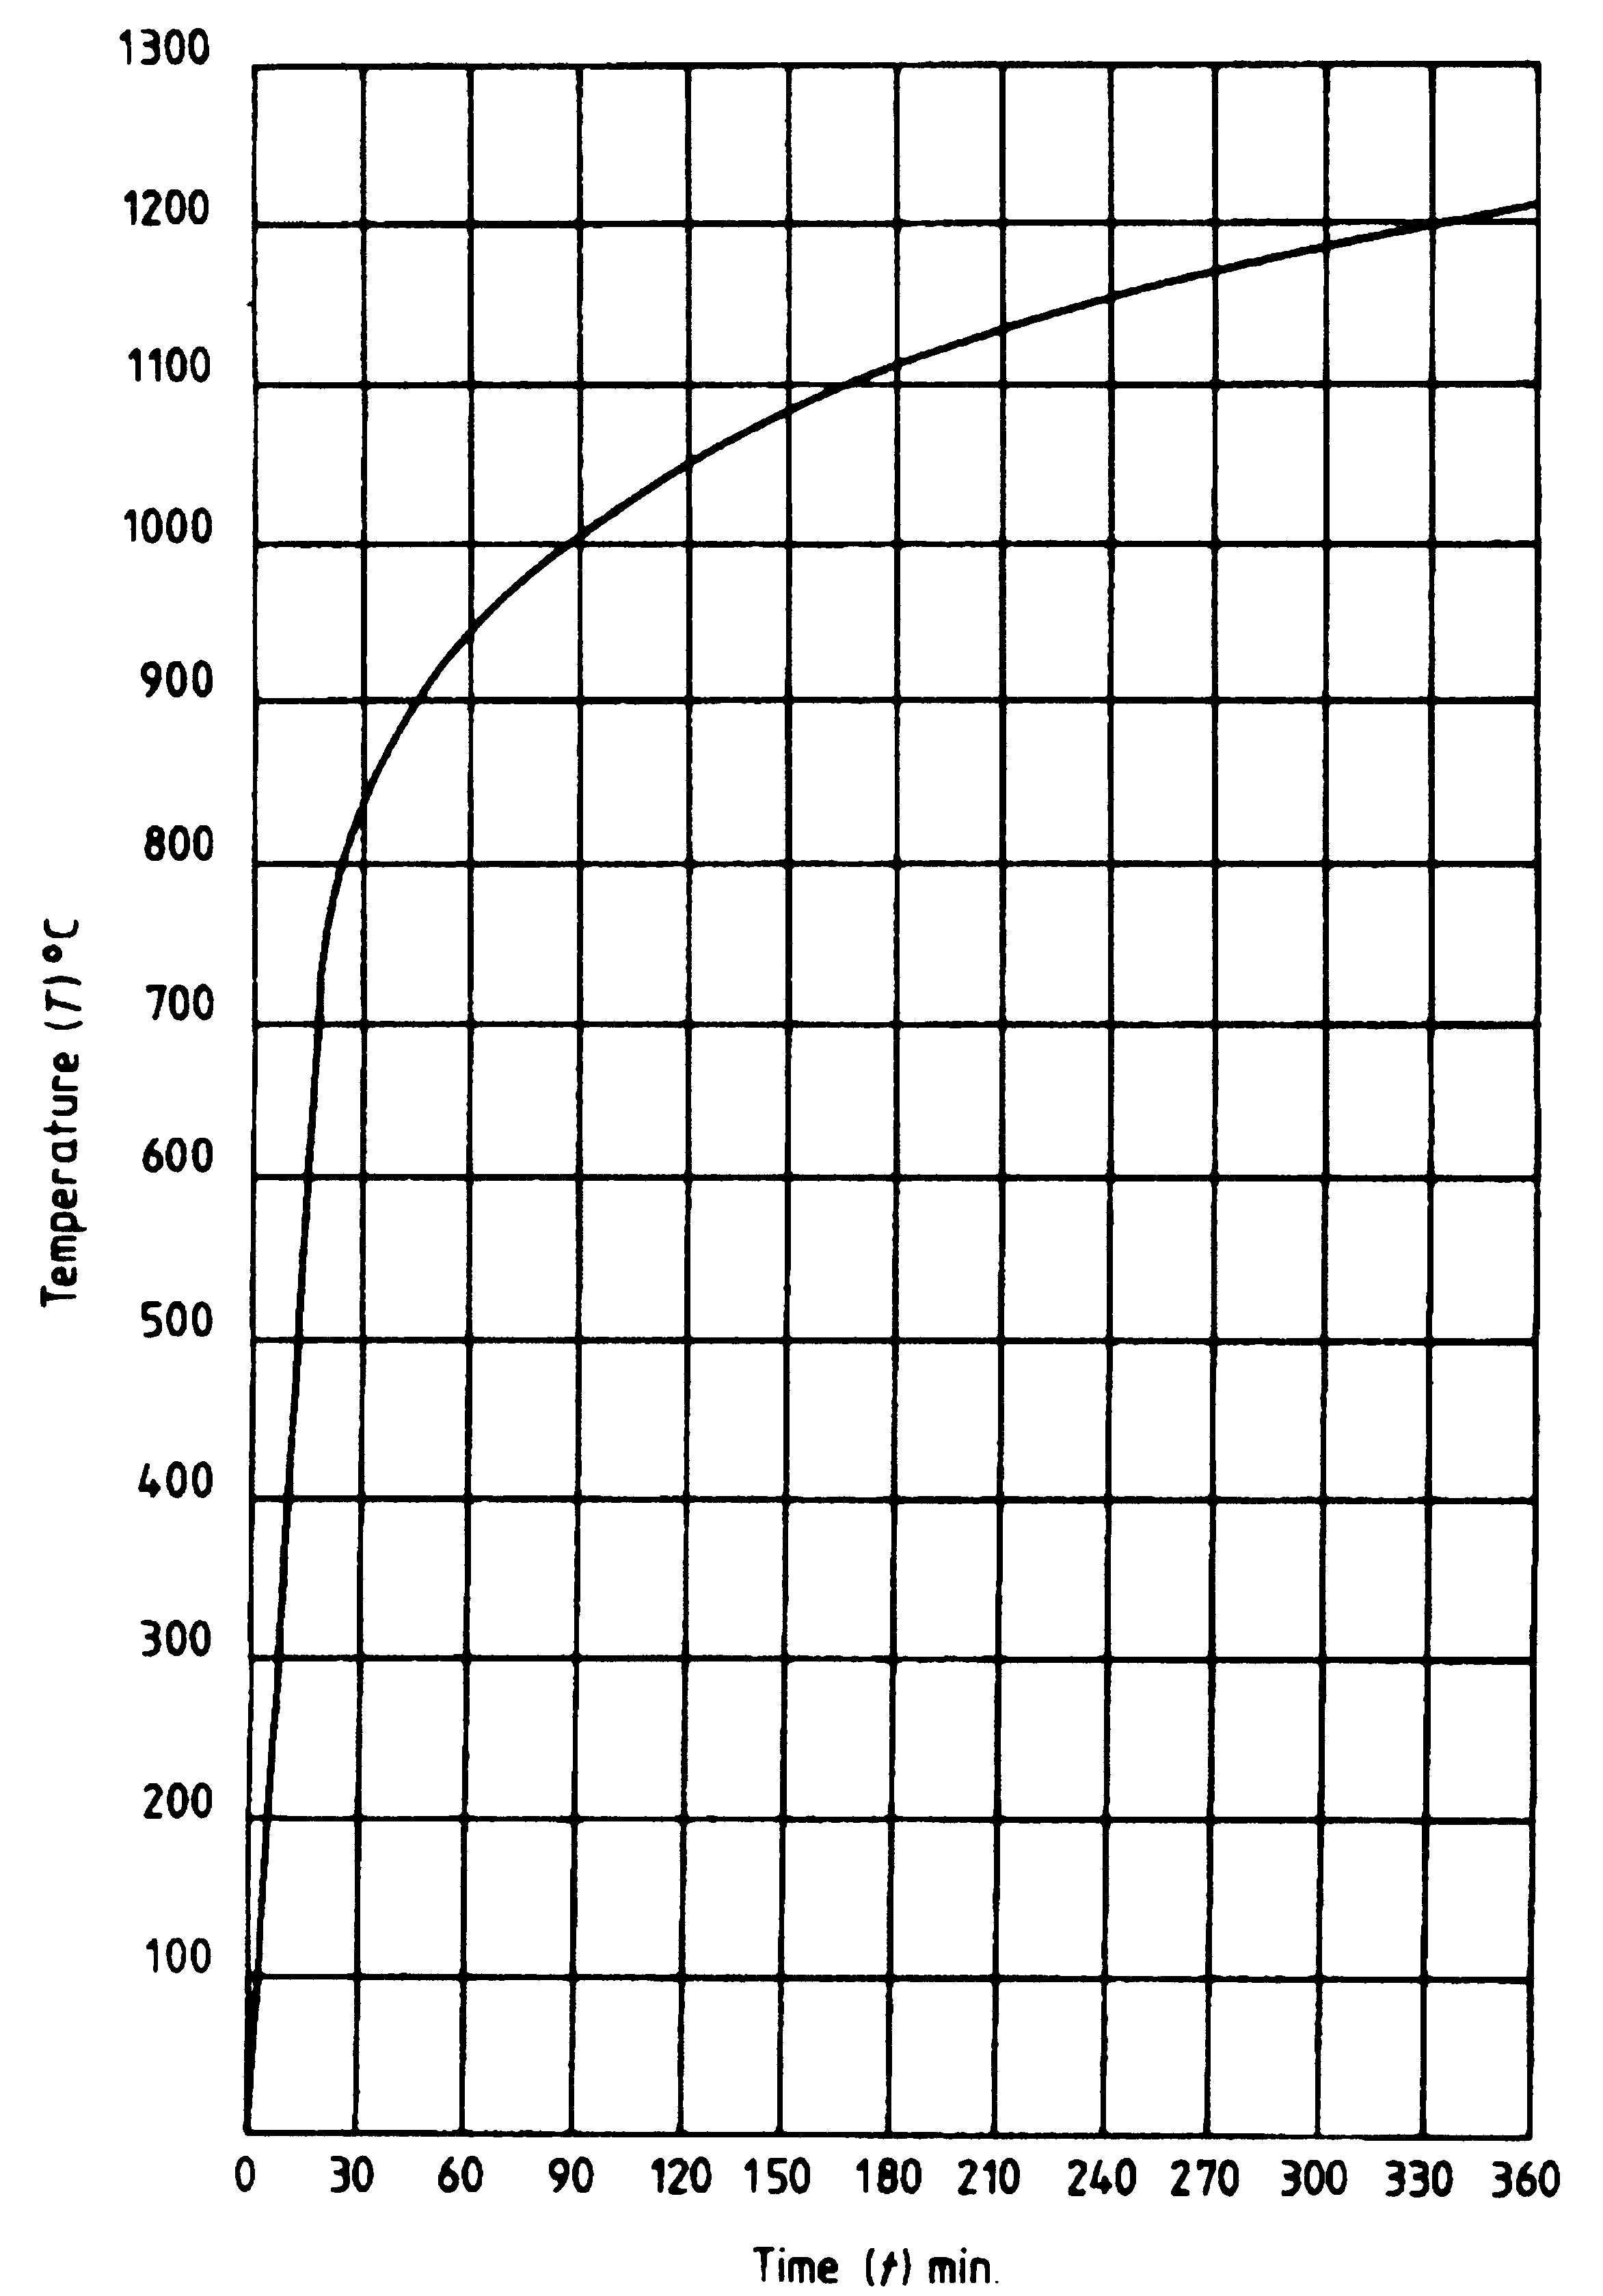
\includegraphics[height=250px]{./Pics/Fire_Curve}
 \end{center}
  \caption{Fire Test Curve}
  \label{fig:Fire Test Curve}
\end{figure}
\\
The fire tests use a specific burning regime within the furnace. As shown in Figure \ref{fig:Fire Test Curve} \citep{BSI476}, the fire curve increases sharply and the temperature gradually increases until the material fails the test. 
\begin{figure}[h]
 \begin{center}
  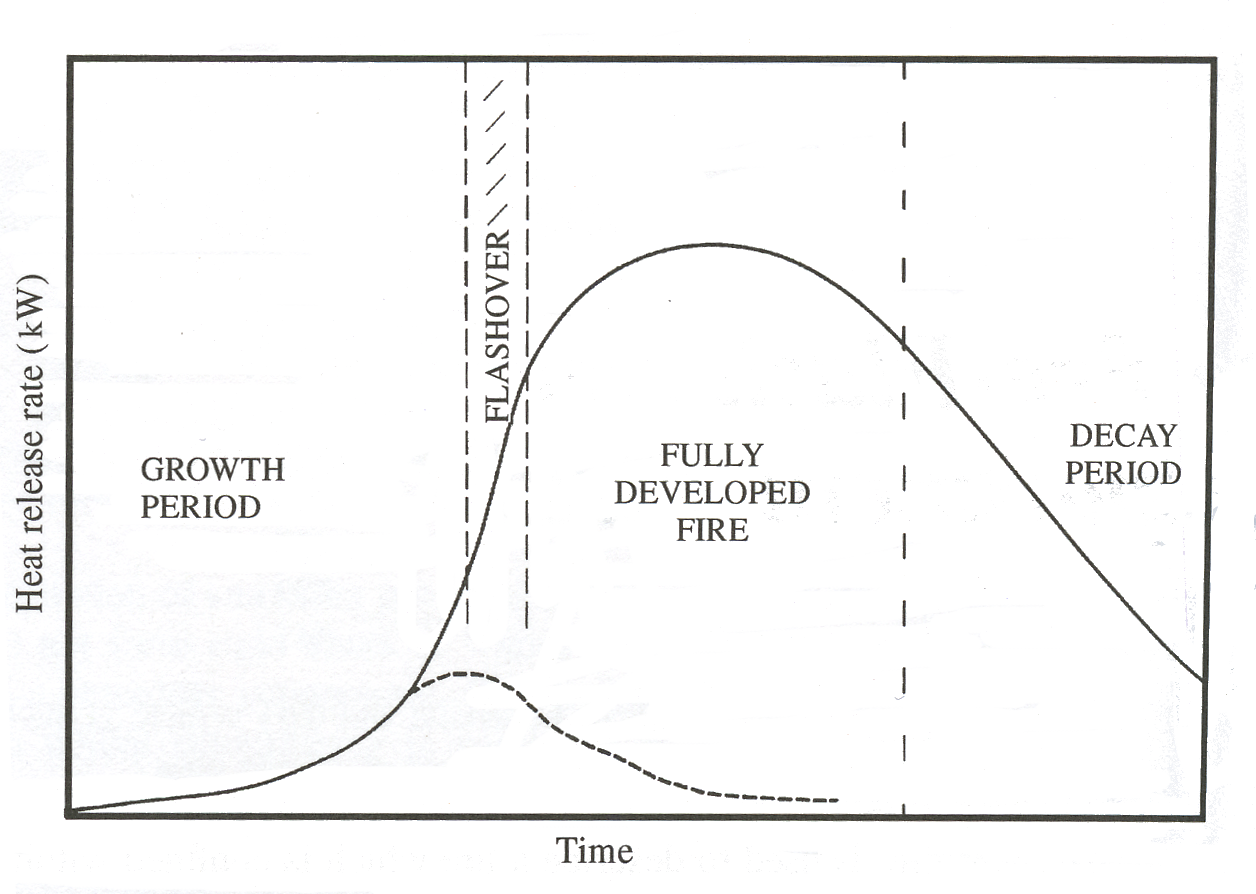
\includegraphics[width=300px]{./Pics/Normal_Fire}
 \end{center}
  \caption{Fire Growth Curve}
  \label{fig:Fire Growth Curve}
\end{figure}
The sharp rise in fire temperature is supposed to represent the increase in fire temperature. However this fire curve does not follow the standard fire growth curve, shown in Figure \ref{fig:Fire Growth Curve} \citep{Drysdale1998}. This has led to research into the fire tests to see if the fire curve provide the correct value for fire resistance values.
\\
\\
In his paper, ``Predicting Fire Resistance Performance of Drywall Construction Exposed to Parametric Design Fires -- A Review'', Nyman looks at the failure of dry wall constructions within a fire scenario and compares the data to the fire resistance rating that the drywall material achieved in a furnace test \citep{JonathanF.Nyman05012008}. He concludes that a fire resistant construction may fail earlier in a real fire situation than suggested by the fire resistance values the material achieved in the fire resistance tests. This early failure may lead to more rapid fire spread than designed for in the building plans and therefore cause issues with the occupants being able to evacuate. Nyman has put forward a differing system for testing drywall construction which is based on the cumulative radiant energy the wall is subjected to in a fire. This different fire testing strategy would more closely model the amount of heat that the construction would suffer from in a fire and therefore give a more accurate fire resistance value.
\subsubsection{Views on Performance Based Engineering}
Not everyone in the fire engineering, construction and architecture trade think that performance based fire engineering is the way forward for fire safety. However these are in the minority. In a study in Hong Kong, Lo found that 71\% of building officials interviewed, thought that fire engineering was necessary to provide reasonable levels of fire protection and life-safety in our rapidly changing environment \citep{Lo2002}. This is also the case in a study of American building officials undertaken by Rickley where 70\% of people agree that fire engineering were essential \citep{Rickley1996}.
\\
In the UK, the release of BS 9999 has opened up the debate on performance based fire engineering with mixed reviews from various people involved in the use of the code. A conference at BRE in Watford on 2\textsuperscript{nd} November 2009 allowed various users of BS 9999 from different areas of the construction industry to air their views on the new standard a year after it was released.
Views on the standard differ but the underlying view was that the code is a step forward in respect to fire design. In his presentation, Andrew Hedges of Arup fire expressed a concern that it could possibly reduce the scope for fire engineering \citep{Hedges2009}. The use of BS 9999 is based on the principles of fire engineering but it does cut down on the need for fire engineering for the majority of buildings as once you have constructed the risk profile of a building (taken from the buildings use and the quantity and type of flammable materials), the process for setting out the required fire safety measures are straightforward and prescriptive to that \emph{specific} risk profile. This means that buildings are tailored to suit the purpose that they were built for - this however may, in the future, cause problems if there is a change of use within the building. Having the building designed to suit can provide cost savings over more restrictive codes and can offer building benefits to those willing to implement sprinkler systems and better building management.
\\
\\
At the same BRE conference, Glyn Jones from the Approved Inspector Services gave the overall view that Approved Inspectors did prefer BS 9999 over the older codes as it ``normalises common sense'' \citep{Jones2009}. Previous codes have allowed the designers to submit building plans that don't follow the building codes but can be proven to be safe. However the final acceptance of the submitted plans is upto the approved inspectors and as they are approving designs that aren't following the building codes, variations in opinions in the inspectors will mean that different plans will be accepted by different inspectors and this leads to variation to the safety measures allowed. However as BS 9999 allows the building fire safety design to be tailored to the building use, the need for fire engineers to provide non code compliant designs will decrease and will therefore mean that the approved inspectors will be able to approve the plans faster and without as much validation.
\\
\\
In a meeting with Mick Green of Buro Happold, concern was raised that the British procedure for fire engineering does not follow the life cycle of a building. The fire engineers are hired during the design phase to design the system and after this, the job is done unless they are hired to also design the management plan or do a risk assessment. Once they have specified the design, the architect or contractor fulfils the procurement phase and purchases the materials for the building based on the fire resistance ratings that the fire engineers have put in the design brief. The materials are then fitted and the fire engineers do not then check that the installed materials and building is what was actually specified. This means that errors could potentially creep into the design between the design specification stage and the final building as Schulz raised \citep{Schulz2009}.
\section{Cost Benefit Analysis and Cost Effectiveness}
The previous section on cost effectiveness and cost benefit analysis focussed on research done specifically on fire engineering methods, this section focuses on methods of cost benefit analysis.
\\
\\
When looking at a system, the costs can be seen as either the costs to build the item and the savings it will make, however for a building, the real costs should focus on the life cycle costs of the item within the building over it's useful lifetime.

\clearpage
\addcontentsline{toc}{section}{Bibliography}
\bibliographystyle{custom}
\bibliography{../../Bibliography} 
\end{document}
